
\chapter{Decidibilità Delle Logiche Modali}


\section{Filtrazione}

Dato una logica $\Lambda$ e una formula a, si può garantire che esiste
un modello $\mu$, con un numero di mondi limitato da f(n), con n
numero di sottoformule di a tale che:

$\teoremaDi{\Lambda}a\iff\vera{\mu}a$

Dimostrazione.

Ip) $a\in\Gamma\implies sottoformule(a)\subseteq\Gamma$

Ts) $\exists\mu:\,\teoremaDi{\Lambda}a\iff\vera{\mu}a$

sia $\mu$=(S,R,V), consideriamo la seguente relazione:

$\sim_{\Gamma}\subseteq S\times S$

che gode della seguente proprietà:

$\Gamma_{\alpha}=\{a\in\Gamma\,|\,\veraw{\mu}{\alpha}a\}$

$\alpha\sim_{\Gamma}\beta\iff\Gamma_{\alpha}=\Gamma_{\beta}$

Si può notare che $\sim_{\Gamma}$ è una relazuione di equivalenza,
Infatti:
\begin{enumerate}
\item è simmetrica\\
$\alpha\sim_{\Gamma}\alpha\iff\Gamma_{\alpha}=\Gamma_{\alpha}$
\item è riflessiva\\
$\alpha\sim_{\Gamma}\beta\iff\Gamma_{\alpha}=\Gamma_{\beta}\iff\beta\sim_{\Gamma}\alpha$
\item è transitiva:\\
$\alpha\sim_{\Gamma}\beta\wedge\alpha\sim_{\Gamma}\gamma\iff\Gamma_{\alpha}=\Gamma_{\beta}=\Gamma_{\gamma}\iff\gamma\sim_{\Gamma}\beta$
\end{enumerate}
Posso allora considerare l'insieme quoziente:

$S_{\Gamma}=S/\sim_{\Gamma}$

Si può dimostrare con il teorema di fattorizzazzione delle applicazioni
che:

$|S_{\Gamma}|\leq2^{|\Gamma|}$

\begin{center} 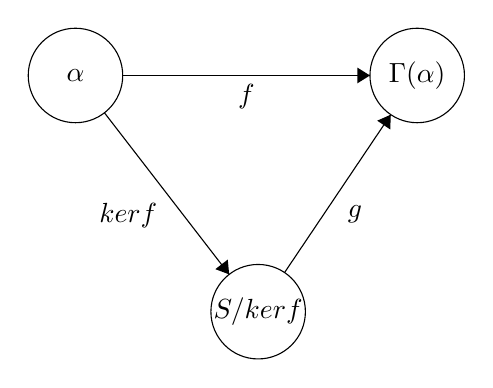
\begin{tikzpicture}[scale=0.2] \tikzstyle{every node}+=[inner sep=0pt] \draw [black] (22.1,-16.4) circle (3); \draw (22.1,-16.4) node {$\alpha$}; \draw [black] (43.8,-16.4) circle (3); \draw (43.8,-16.4) node {$\Gamma(\alpha)$}; \draw [black] (33.7,-31.4) circle (3); \draw (33.7,-31.4) node {$S/kerf$}; \draw [black] (35.38,-28.91) -- (42.12,-18.89); \fill [black] (42.12,-18.89) -- (41.26,-19.27) -- (42.09,-19.83); \draw (39.36,-25.24) node [right] {$g$}; \draw [black] (25.1,-16.4) -- (40.8,-16.4); \fill [black] (40.8,-16.4) -- (40,-15.9) -- (40,-16.9); \draw (32.95,-16.9) node [below] {$f$}; \draw [black] (23.94,-18.77) -- (31.86,-29.03); \fill [black] (31.86,-29.03) -- (31.77,-28.09) -- (30.98,-28.7); \draw (27.33,-25.31) node [left] {$kerf$}; \end{tikzpicture} \end{center}

Per dimostrarlo basta prendere:

$f:\,\alpha\rightarrow\mathcal{P}(\Gamma)$

risulta banale verificare che:

$ker\, f\equiv\sim_{\Gamma}$

e quindi, ricordando che g è iniettiva, risulta banale che:

$|S/\sim_{\Gamma}|\leq\Gamma(\alpha)$

Allora possiamo prendere il modello:

$M^{\Gamma}=(S^{\Gamma},R',V^{\Gamma})$

$R'\subseteq S^{\Gamma}\times S^{\Gamma}$

con R' che soddisfi le seguenti proprietà:

F1) $(\alpha,\,\beta)\in R\implies([\alpha],\,[\beta])\in R'$

F2) $([\alpha],[\beta])\in R'\implies\forall\boxx b\in\Gamma,\,\veraw{\mu}{\alpha}{\boxx b}\implies\veraw{\mu}{\beta}b$

Una relazione che gode delle proprietà F1 e F2 si chiama $\Gamma$-filtrazione
della relazione R.

prendiamo infine:

$V^{\Gamma}:\,\Phi\cap\Gamma\rightarrow\mathcal{P}(S^{\Gamma})$

che gode della seguente proprietà:

presa una formula atomica $A\in\Phi\cap\Gamma$

$\alpha\in V^{\Gamma}(A)\iff\alpha\in V(A)$


\subsection{Teorema}

Esiste almeno una relazione che gode delle proprietà F1 e F2:

$R^{\sigma}\subseteq S^{\Gamma}\times S^{\Gamma}$

così definita:

$([\alpha],[\beta])\in R^{\sigma}\iff\exists\delta\in[\alpha],\eta\in[\beta]\,:\,(\delta,\,\eta)\in R$

La proprietà F1 è dimostrata banalmente.

Dimostriamo F2

Ip) $([\alpha],[\beta])\in R^{\sigma}$, $\boxx{b\in\Gamma}$, $\veraw{\mu}{\alpha}{\boxx b}$

Ts) $R^{\delta}$gode della proprietà F2

supponiamo che:

$\exists\delta,\eta\,:\,\delta R\eta\wedge\delta\in[\alpha]\wedge\eta\in[\beta]$

avremo che:

$\veraw{\mu}{\delta}{\boxx b}$

$\veraw{\mu}{\eta}b$

e quindi:

$\veraw{\mu}{\beta}b$\\



\section{Lemma di Filtrazione}

dato un insieme$\Gamma$ chiuso rispetto alle sottoformule di a, con
$a\in\Gamma$

$\veraw{\mu}{\alpha}{a\iff}\veraw{\mu^{\Gamma}}{\alpha}a$

per ogni $\mu^{\Gamma}$$\Gamma$-filtrazione di $\mu$

Dimostrazione:

Ts) $\veraw{\mu}{\alpha}{a\iff}\veraw{\mu^{\Gamma}}{[\alpha]}a$

Ip) $\mu^{\Gamma}$$\Gamma$-filtrazione di $\mu$

Per induzione sul numero di connettivi di a

Caso Base, n=0:

a non ha connettivi, allora $a\equiv A$

$\veraw{\mu}{\alpha}A\iff\alpha\in V(A)\iff\alpha\in V^{\Gamma}(A)\iff\veraw{\mu^{\Gamma}}{[\alpha]}a$

Ipotesi di induzione: il teorema vale per ogni formula di $\Gamma$
con m<n connettivi.

a può essere:
\begin{enumerate}
\item $\neg b$
\item $b\implies c$
\item $\boxx b$
\end{enumerate}
Caso 1:

$\veraw{\mu}{\alpha}{\neg b}\iff\nonveraw{\mu}{\alpha}b\iff\nonveraw{\mu^{\Gamma}}{[\alpha]}b\iff\veraw{\mu^{\Gamma}}{[\alpha]}{\neg b}$

Caso 2:

$\veraw{\mu}{\alpha}{b\implies c}$ se e solo se $\nonveraw{\mu}{\alpha}b$
oppure $\veraw{\mu}{\alpha}c$

quindi si può affermare

$\nonveraw{\mu}{\alpha}b\iff\nonveraw{\mu^{\Gamma}}{[\alpha]}b$

$\veraw{\mu}{\alpha}c\iff\veraw{\mu^{\Gamma}}{[\alpha]}c$

ma vale almeno una delle due se e solo se

$\veraw{\mu^{\Gamma}}{[\alpha]}{b\implies c}$

Caso 3:

Ip) $\veraw{\mu}{\alpha}{\boxx b}$

Ts) $\veraw{\mu^{\Gamma}}{[\alpha]}{\boxx b}$

Consideriamo la reazione R' avente le proprietà F1 e F2

$\forall[\beta]\,:\,([\alpha],\,[\beta])\in R'\implies\veraw{\mu^{\Gamma}}{[\beta]}b$
-- per F2

allora si può affermare che:

$\veraw{\mu}{\beta}b\implies\veraw{\mu^{\Gamma}}{[\beta]}b\implies\veraw{\mu^{\Gamma}}{[\alpha]}{\boxx b}$

Ip)$\veraw{\mu^{\Gamma}}{[\alpha]}{\boxx b}$

Ts)$\veraw{\mu}{\alpha}{\boxx b}$

$\forall[\beta]\,:\,(\alpha,\,\beta)\in R,\,([\alpha],\,[\beta])\in R'$
--per F1

allora si può affermare che:

$\veraw{\veraw{\mu^{\Gamma}}{[\beta]}b\implies\mu}{\beta}b\implies\veraw{\mu}{\alpha}{\boxx b}$


\section{Determinatezza di K dai Frame Finiti}

La minima logica normale K è determinata dalla classe di tutti i frame
finiti.

Se $a$ ha n sottoformule $a$ è un teorema di K se e solo se A è
valida in tutti i frame con meno di $2^{n}$ mondi. 

$\teoremaDi Ka$ se e solo se $\vera Fa$.\\


Ip)$\teoremaDi Ka$ 

Ts)$\vera Fa$\\


Se $a$ è un teorema di K allora $a$ è valida in tutti i frame (infatti
K è determinata rispetto alla classe di tutti i frame) è a maggior
ragione valida in tutti i frame finiti ed in tutti i frame con meno
di $2^{n}$ mondi.\\


Ip)$\vera Fa$

Ts)$\teoremaDi Ka$\\
\\
Suppongo per assurdo che$\nonTeor Ka$ se e solo se $\nonvera{M^{K}}a$
se e solo se (per il lemma di filtrazione) $\nonvera{(M^{K})^{\Gamma}}a$
il che implica che

in particolare $\nonvera{(F^{K})^{\Gamma}}a$ dove $(F^{K})^{\Gamma}$
è il Frame su cui è costruita la filtrazione del modello canonico
costruito rispetto alla logica $K$ 

Si noti che $(M^{K})^{\Gamma}$ ha al più $2^{n}$ mondi.


\section{Determinatezza di KD dai Frame seriali finiti}

Per seguire lo stesso ragionamente della dimostrazione appena fatta,
dobbiamo solo mostrare che se $R$ è seriale allora $R^{\sigma}$
lo è.\\


\ovalbox{\begin{minipage}[t]{1\columnwidth}%
\textbf{Nota:}$R^{\sigma}\subseteq S^{\Gamma}\times S^{\Gamma}$

così definita:

$([\alpha],[\beta])\in R^{\sigma}\iff\exists\delta\in[\alpha],\eta\in[\beta]\,:\,(\delta,\,\eta)\in R$%
\end{minipage}}\\
\\
Sia $[\alpha]\in S^{\Gamma}$

Se $R^{KD}$ è seriale allora $\forall\delta\in S^{KD}\exists\eta\in S^{KD}:\ (\delta,\eta)\in R^{KD}$

In particolare esiste$\delta$ appartiene alla classe di equivalenza
$[\alpha]$ (di cui al limite potrebbe essere l'unico elemento con
$\alpha=\delta$)

Dalla serialità abbiamo che esiste$\eta$ appartiene alla classe di
equivalenza $[\beta]$

Da cui $([\alpha],[\beta])\in R^{\sigma}$


\section{Determinatezza di K4 dai Frame transitivi finiti}

L'aspetto interessante di questa dimostrazione sta nel fatto che non
possiamo usare la relazione ``classica'' $R^{\sigma}$ come $\Gamma$-filtrazione
ma dobbiamo costruirne una ad hoc, dato che se $R^{K4}$ è transitiva
la sua filtrazione standard non è detto che lo sia

Definiamo quindi $R^{\tau}$così:

$([\alpha],[\beta])\in R^{\tau}$ se se e solo se per ogni fbf $b$,
$\boxx b\in\Gamma$ e $\vera M{_{\alpha}\boxx b}$ implicano $\vera M{_{\beta}b\wedge\boxx b}$

dimostriamo che $R^{\tau}$ è una $\Gamma$-filtrazione transitiva\\


$R^{\tau}$è una $\Gamma$-filtrazione\\


F2) $([\alpha],[\beta])\in R^{\tau}$ se e solo se$\vera M{_{\alpha}\boxx b}$
implicano $\vera M{_{\beta}b\wedge\boxx b}$ da cui: $\{b\ |\ \boxx{b\in\alpha\}\subseteq\beta}$
e quindi $\alpha,\beta\in R^{K4}$

F1) $(\alpha,\beta)\in R^{K4}$per ogni $\boxx{b\in\Gamma}$, se $\vera M{_{\alpha}\boxx b}$
allora anche (schema 4) $\veraw M{\alpha}{\boxx{\boxx b}}$ 

dato che $(\alpha,\beta)\in R^{K4}$ , anche:

$\veraw M{\beta}b$ e $\veraw M{\beta}{\boxx b}$ e quindi:

$\veraw M{\beta}{b\wedge\boxx b}$\\


$R^{\tau}$ è transitiva\\


Sia $([\alpha],[\beta])\in R^{\tau}$, $([\beta],[\gamma])\in R^{\tau}$
ora la prima implica che per ogni fbf $b$, da $\boxx{b\in\Gamma}$
e $\veraw M{\alpha}{\boxx b}$ segua $\vera M{_{\beta}\boxx{b\wedge b}}$,
e da questa essendo $([\alpha],[\beta])\in R^{\tau}$, segue anche
$\vera M{_{\gamma}\boxx{b\wedge b}}$, cioè $([\beta],[\gamma])\in R^{\tau}$


\section{Tableaux}

I Tableaux sono un metodo efficiente per dimostrare la verità, falsità
e soddisfacibilità di una formula

Il metodo consiste nel partire dalla formula che si vuole considerare,
negandola.

Dopodichè si procede passo passo alla costruzione di un albero seguendo
delle regole di espansione che aggiungono uno o più nodi o rami all'albero.

Le regole con la virgola aggiungono un nodo allo stesso ramo, mentre
le regole con il pipe sdoppiano il ramo.

Se espando una formula, devo aggiungere coerentemente l'espansione
a tutti i sottorami, e non posso più espanderla.

Se un cammino contiene sia una formula che la sua negazione il cammino
si chiude.

Se esiste almeno un cammino chiuso, la formula di partenza è soddisfacibile,
se tutti i cammini sono chiusi, la formula è logicamente valita, altrimenti
la formula è falsa.


\subsection{Tableaux per la logica proposizionale}

Le regole Per applicare l'algoritmo dei tableaux nella logica proposizionale
sono le seguenti:
\begin{itemize}
\item Radice dell'albero\\
$\neg a$
\item Regola del $\neg$\\
$\dfrac{\neg\neg a}{a}$
\item Regole di tipo $\alpha$\\
$\dfrac{a\wedge b}{a,\, b}$ $\dfrac{\neg(a\vee b)}{\neg a,\,\neg b}$
$\dfrac{\neg(a\implies b)}{a,\,\neg b}$
\item Regole di tipo $\beta$\\
$\dfrac{a\vee b}{a|b}$ $\dfrac{\neg(a\wedge b)}{\neg a|\neg b}$
$\dfrac{a\implies b}{\neg a|b}$
\item Regole di tipo $\iff$\\
$\dfrac{a\iff b}{a,\, b|\neg a,\,\neg b}$ $\dfrac{\neg(a\iff b)}{a,\,\neg b|\neg a,\, b}$
\end{itemize}

\subsection{Tableaux per le logiche modali}

Per le logiche modali, si può modificare l'algoritmo già usato per
le logiche proposizionali, aggiungendo le regole per la necessitazione
e considerando che ogni regola deve essere vera in un mondo.

Per fare ciò devo aggiungere l'indice del mondo a tutte le regole,
e si potrà chiudere un ramo solo se si trova la regola e il suo negato
nello stesso mondo.

Le regole dei tableaux per le logiche modali saranno:
\begin{itemize}
\item Radice dell'albero\\
$1.\neg a$
\item Regola del $\neg$\\
$\dfrac{\delta\,\neg\neg a}{\delta a}$
\item Regole di tipo $\alpha$\\
$\dfrac{\delta\, a\wedge b}{\delta\, a,\,\delta\, b}$ $\dfrac{\delta\,\neg(a\vee b)}{\delta\,\neg a,\,\delta\,\neg b}$
$\dfrac{\delta\,\neg(a\implies b)}{\delta\, a,\,\delta\,\neg b}$
\item Regole di tipo $\beta$\\
$\dfrac{\delta\, a\vee b}{\delta\, a|\delta\, b}$ $\dfrac{\delta\,\neg(a\wedge b)}{\delta\,\neg a|\delta\,\neg b}$
$\dfrac{\delta\, a\implies b}{\delta\,\neg a|\delta\, b}$
\item Regole di tipo $\iff$\\
$\dfrac{\delta\, a\iff b}{\delta\, a,\,\delta\, b|\delta\,\neg a,\,\delta\,\neg b}$
$\dfrac{\delta\,\neg(a\iff b)}{\delta\, a,\,\delta\,\neg b|\delta\,\neg a,\,\delta\, b}$
\item Regole di necessitazione\\
$\dfrac{\sigma\,\boa}{\sigma_{n}\, a}$ $\dfrac{\sigma\,\neg\dia}{\sigma_{n}\,\neg a}$
-- con $\sigma_{n}$ già presente nei nodi precedenti\\
$\dfrac{\sigma\,\neg\boa}{\sigma_{n}\,\neg a}$ $\dfrac{\sigma\,\dia}{\sigma_{n}\, a}$
-- con $\sigma_{n}$ non presente nei nodi precedenti
\end{itemize}
Tuttavia queste regole non sono sufficienti se vogliamo usare una
regola modale differente da K.

Per lavorare su regole con proprietà dei frame particolari, devo necessariamente
cambiare le regole di necessitazione aggiungendo dei vincoli alla
generazione di nuovi mondi in modo tale che rispettino le proprietà
del frame.


\section{Logiche notevoli}

Abbiamo visto K essere la logica modale minima, a partire da questa
logica ne possiamo ottenere altre aggiungendo ad essa alcuni schemi
di assiomi:
\begin{itemize}
\item D : $\boa\implies\dia$ (seriale)
\item T: $\boa\implies a$ (riflessiva)
\item B: $a\implies\boxx{\dia}$ (simmetrica)
\item 4:$\boa\implies\boxx{\boa}$ (transitiva)
\item 5: $\diam a\implies\boxx{\diam a}$ (euclidea)
\end{itemize}
Per ognuno di questi schemi di assiomi (X) ne esiste il cosiddetto
duale (X$\diamond$), cioè lo schema che si ottine invertendo antecedente
e conseguente e negando $\boxx a$ con $\dia$


\subsection{Teorema: validità del duale }

M sia una sequenza di connettivi $\square$, $\diamond$ ed M' il
suo duale.

Idem per N ed N'.\\


Ip) $Ma\implies Nb$

Ts) $N'b\implies M'a$\\


Se vale lo schema d'assiomi $Ma$ deve valere anche $M\neg a$ dato
che appunto è uno schema.

Riscrivo l'ipotesi come:

$M\neg a\implies N\neg b$

Considero la tautologia della PL: $(C\implies D)\implies(\neg D\implies\neg C)$

la applico all'ipotesi ottenendo:

$(M\neg a\implies N\neg b)\implies(\neg(N\neg b)\implies\neg(M\neg a))$

Da cui per MP con l'ipotesi (riscritta) ottengo:

$\neg(N\neg b)\implies\neg(M\neg a)$

Usando ripetutamente le equivalenze tra$\square$ e $\diamond$ ottengo:

$N'\neg\neg b\implies M'\neg\neg a$ semplificando:

$N'b\implies M'a$

La dimostrazione nell'altro senso è del tutto simmetrica dato che
le operazioni effettuate sono valide in entrambe le direzioni


\subsection{Esempio validità del duale: schema 5}

Ip) $\diam a\implies\boxx{\diam a}$

Ts)$\diamond\boxx a\implies\boxx a$\\


Riscrivo l'ipotesi come:

$\diam{\neg a}\implies\boxx{\diam{\neg a}}$

Considero la tautologia della PL: $(C\implies D)\implies(\neg D\implies\neg C)$

$(\diam{\neg a}\implies\boxx{\diam{\neg a}})\implies(\neg\boxx{\diam{\neg a}}\implies\neg\diam{\neg a})$

Semplifico il conseguente :$\neg\boxx{\diam{\neg a}}\implies\neg\diam{\neg a}$
diventa

$\diam{\square\neg\neg a\implies\square\neg\neg a}$ , semplificando
i $\neg$:

$\diam{\square a\implies\square a}$

Cioè la tesi.\\


Vogliamo ora mostrare come alcune notazione della forma KX denotino
la stessa logica.

Ricordiamo che con KX intendiamo la logica K a cui abbiamo aggiunto
il generico assioma X

KB4 = K + assioma B + assioma 4


\subsection{Inclusione di KD in KT}

Pare ovvio che una logica riflessiva sia anche seriale (se parlo da
solo parlo con qualcuno), ma dimostriamolo comunque. \\


Ip) KT

Ts) KD\\
Se vale T: 

$\boa\implies a$ (riflessiva)

allora vale anche il suo duale $T\diamond$:

$a\implies\dia$

Per la catena di implicazioni $(\implica ab,\ \implica bc,\ \mbox{\ensuremath{\implica ac}})$
abbiamo:

$\boa\implies\dia$

Cioè lo schema D\\


\textbf{Lemma implica in KB:}

IP)$\teoremaDi{KB}\diamond C\implies D$

TS) $\teoremaDi{KB}\implica C{\boxx D}$\\


Per Ip) $\diamond C\implies D$ e quindi, dato che è un teorema della
logica KB, (che è una logica normale)

posso usare la definizione 3 equivalente di logica normale ottenendo:

$\square\diamond C\implies\square D$ 

Inoltre vale lo schema B

$C\implies\boxx{\diam C}$

Leggendo i due schemi appena scritti dal secondo al primo riconosciamo
la catena di implicazioni $(\implica ab,\ \implica bc,\ \mbox{\ensuremath{\implica ac}})$ 

Da cui: $C\implies\boxx D$


\subsection{Equivalenza KB4, KB5}

\textbf{Da KB4 a KB5}

Valendo 4 vale anche 4$\diamond$:

$\diamond(\dia)\implies(\diamond a)$, e tenendo conto del precedente
lemma 

(dove $C$ è $\diamond a$ e $B$ è $\diamond a$), 

abbiamo $\diamond a\implies\boxx{\dia}$ cioè lo schema5. \\


\textbf{Da KB5 a KB4}

Da 5 infatti deduciamo 5$\diamond$: $\diam{(\square a)\implies(\boa)}$

Tenuto conto della prima osservazione (con$C$ e$B$ uguali ad $a$)

abbiamo $\boa\implies\boxx{\boa}$.\\



\subsection{Equivalenza KDB4. KDB5, KDB45, KTB4, KT5}

\textbf{KDB4 = KDB5 = KD45}, infatti aggiungendo l'assioma D a due
logiche equivalenti (KB4, KB5) continuano a rimanere equivalenti;

aggiungere 4 a KDB5 non produce alcun effetto perché lo contiene già.\\


Inoltre notiamo che: \textbf{KDB4$\subseteq$KTB4} in quanto KT contiene
KD

e \textbf{KT5$\subseteq$KTB4} in quando KT4B contiene KT4 che coincide
con KT5.\\


Mostriamo che \textbf{KTB4$\mbox{\ensuremath{\subseteq}}$KDB4 }così
da arrivare a KTB4 = KDB4

Cioe' mostriamo che nella logica K, dall'assioma T, con B e 4 posso
dedurre l'assioma D

Dall'assioma T deduciamo l'assioma T$\diamond$ cioe' $a\implies\diamond a$

Dato che vale 5: $\diam a\implies\boxx{\diam a}$, sfruttando la catena
di implicazioni delle due precedenti abbiamo:

$a\implies\boxx{\dia}$ cioè B.\\



\subsection{Reticolo delle logiche}

\begin{center} 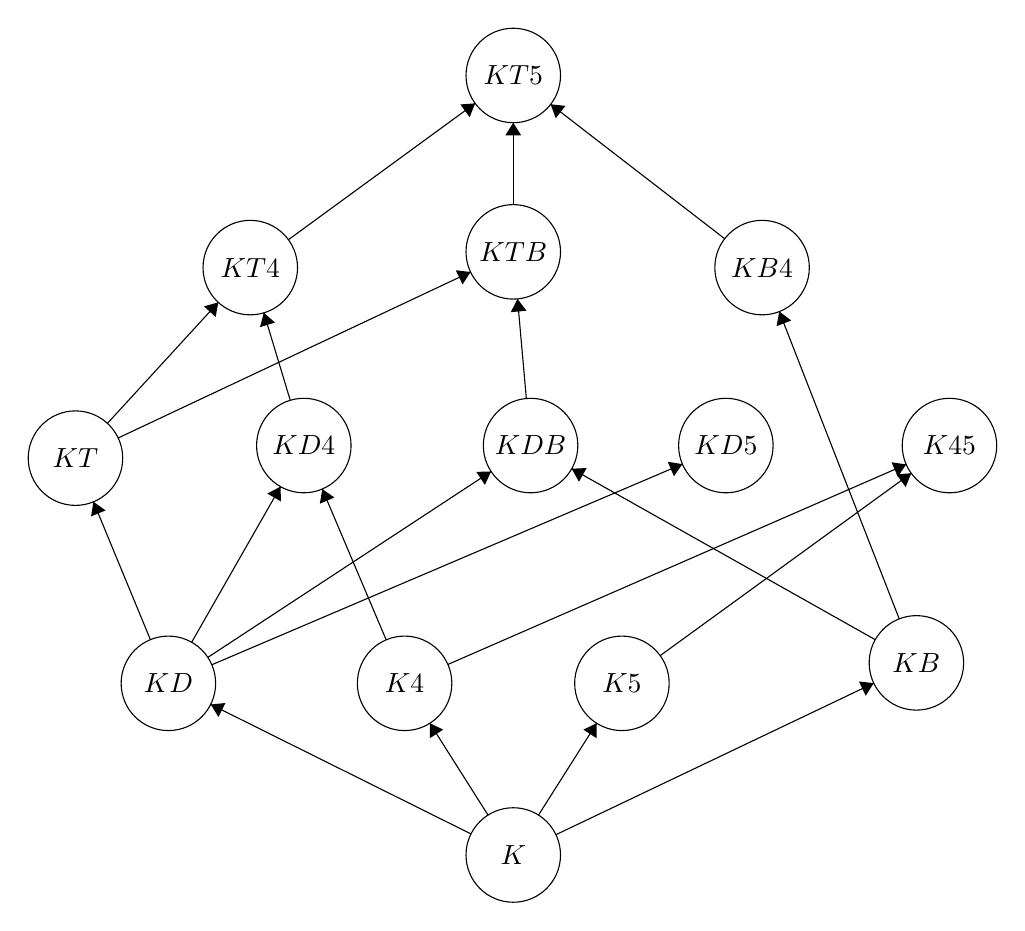
\begin{tikzpicture}[scale=0.2] \tikzstyle{every node}+=[inner sep=0pt] \draw [black] (39.9,-53.7) circle (3); \draw (39.9,-53.7) node {$K$}; \draw [black] (18,-42.8) circle (3); \draw (18,-42.8) node {$KD$}; \draw [black] (33,-42.8) circle (3); \draw (33,-42.8) node {$K4$}; \draw [black] (65.5,-41.5) circle (3); \draw (65.5,-41.5) node {$KB$}; \draw [black] (46.8,-42.8) circle (3); \draw (46.8,-42.8) node {$K5$}; \draw [black] (12.1,-28.5) circle (3); \draw (12.1,-28.5) node {$KT$}; \draw [black] (26.6,-27.7) circle (3); \draw (26.6,-27.7) node {$KD4$}; \draw [black] (53.4,-27.7) circle (3); \draw (53.4,-27.7) node {$KD5$}; \draw [black] (67.6,-27.7) circle (3); \draw (67.6,-27.7) node {$K45$}; \draw [black] (23.2,-16.4) circle (3); \draw (23.2,-16.4) node {$KT4$}; \draw [black] (39.9,-15.4) circle (3); \draw (39.9,-15.4) node {$KTB$}; \draw [black] (55.7,-16.4) circle (3); \draw (55.7,-16.4) node {$KB4$}; \draw [black] (39.9,-4.2) circle (3); \draw (39.9,-4.2) node {$KT5$}; \draw [black] (41,-27.7) circle (3); \draw (41,-27.7) node {$KDB$}; \draw [black] (37.21,-52.36) -- (20.69,-44.14); \fill [black] (20.69,-44.14) -- (21.18,-44.94) -- (21.62,-44.05); \draw [black] (38.3,-51.17) -- (34.6,-45.33); \fill [black] (34.6,-45.33) -- (34.61,-46.28) -- (35.45,-45.74); \draw [black] (42.61,-52.41) -- (62.79,-42.79); \fill [black] (62.79,-42.79) -- (61.85,-42.68) -- (62.28,-43.59); \draw [black] (41.5,-51.17) -- (45.2,-45.33); \fill [black] (45.2,-45.33) -- (44.35,-45.74) -- (45.19,-46.28); \draw [black] (16.86,-40.03) -- (13.24,-31.27); \fill [black] (13.24,-31.27) -- (13.09,-32.2) -- (14.01,-31.82); \draw [black] (14.13,-26.29) -- (21.17,-18.61); \fill [black] (21.17,-18.61) -- (20.26,-18.86) -- (21,-19.54); \draw [black] (25.74,-24.83) -- (24.06,-19.27); \fill [black] (24.06,-19.27) -- (23.82,-20.18) -- (24.77,-19.89); \draw [black] (31.83,-40.04) -- (27.77,-30.46); \fill [black] (27.77,-30.46) -- (27.62,-31.39) -- (28.54,-31); \draw [black] (19.48,-40.19) -- (25.12,-30.31); \fill [black] (25.12,-30.31) -- (24.28,-30.75) -- (25.15,-31.25); \draw [black] (20.76,-41.62) -- (50.64,-28.88); \fill [black] (50.64,-28.88) -- (49.71,-28.73) -- (50.1,-29.65); \draw [black] (35.75,-41.6) -- (64.85,-28.9); \fill [black] (64.85,-28.9) -- (63.92,-28.76) -- (64.32,-29.68); \draw [black] (49.23,-41.04) -- (65.17,-29.46); \fill [black] (65.17,-29.46) -- (64.23,-29.53) -- (64.82,-30.34); \draw [black] (64.41,-38.71) -- (56.79,-19.19); \fill [black] (56.79,-19.19) -- (56.62,-20.12) -- (57.55,-19.76); \draw [black] (62.89,-40.03) -- (43.61,-29.17); \fill [black] (43.61,-29.17) -- (44.07,-30) -- (44.56,-29.13); \draw [black] (20.51,-41.15) -- (38.49,-29.35); \fill [black] (38.49,-29.35) -- (37.55,-29.37) -- (38.1,-30.2); \draw [black] (14.81,-27.22) -- (37.19,-16.68); \fill [black] (37.19,-16.68) -- (36.25,-16.57) -- (36.68,-17.47); \draw [black] (40.73,-24.71) -- (40.17,-18.39); \fill [black] (40.17,-18.39) -- (39.74,-19.23) -- (40.74,-19.14); \draw [black] (25.62,-14.63) -- (37.48,-5.97); \fill [black] (37.48,-5.97) -- (36.54,-6.04) -- (37.13,-6.85); \draw [black] (39.9,-12.4) -- (39.9,-7.2); \fill [black] (39.9,-7.2) -- (39.4,-8) -- (40.4,-8); \draw [black] (53.33,-14.57) -- (42.27,-6.03); \fill [black] (42.27,-6.03) -- (42.6,-6.92) -- (43.21,-6.13); \end{tikzpicture} \end{center}

\textbf{\large{Somma diretta di Frame}}\textbf{}\\


S5 è determinata dalla classe dei frame d’ equivalenza (cioè frame
in cui la relazione di accessibilità è una relazione di equivalenza),
S5 = KT5 = KTB4 (riflessiva, simmetrica, transitiva)

S5 è determinata dalla classe dei frame universali (cioè frame in
cui la relazione di accessibilità è la relazione universale).

Mostriamo (almeno argomentiamo) la seconda affermazione.\\


Data una collezione di frame con insiemi di mondi a due a due disgiunti,
si dice somma diretta di questi frame il frame che ha come insieme
dei mondi l’unione dell’insieme dei mondi dei frame della collezione
e come relazione la unione delle relazioni dei frame della collezione.

$F=(S,R)$

$F1=(S1,R1)$, $F2=(S2,R2)$

$F=F1\oplus F2$ se e solo se $F=(S1\cup S2,\ R1\cup R2)$

Si dimostra che $\vera Fa$ se e solo se $\vera{F1}a$ e $\vera{F2}a$

Dato che una relazione di equivalenza forma una partizione sull'insieme
su cui è definita, e che in ogni classe di equivalenza è una relazione
universale, possiamo vedere una relazione di equivalenza come somma
di relazioni universali e il suo insieme come somma disgiunta di insiemi;
la somma diretta pertanto ci mostra quindi che S5 è determinata dai
frame universali.


\subsection{Tableau rivisitato per KT, KB}

Se una logica contiene l'assioma B devo aggiungere alle regole del
Tableau
\begin{itemize}
\item Regole di necessitazione\\
$\dfrac{\sigma\,\boa}{\sigma_{n}\, a}$ $\dfrac{\sigma\,\neg\dia}{\sigma_{n}\,\neg a}$
-- con $\sigma_{n}$ già presente nei nodi precedenti, oppure $\sigma_{n}$
\textbf{nodo corrente}
\end{itemize}
es. Si provi che la formula: $(\boa\implies a)$ è un teorema in KB

1: $\neg(\boa\implies a)$

1: $\boa$

1: $\neg a$

\textbf{1}: $a$ 

\begin{center}
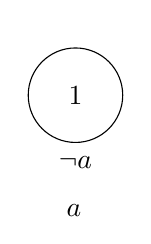
\begin{tikzpicture}[scale=0.2] 
\tikzstyle{every node}+=[inner sep=0pt] 
\draw [black] (26.8,-10.8) circle (3);
\draw (26.8,-10.8) node {1}; 

 
\draw (26.8,-6.6) node {$\boa$}; 

\draw (26.8,-15.1) node {$\neg{a}$};

\draw (26.7,-18.1) node {$a$}; 


\end{tikzpicture}
\end{center} 

Dove nell'ultimo passaggio ho usato proprio la regola appena introdotta,
avendo ottenuto $a$ e $\neg a$ nello stesso stato (mondo) deduco
che negare $a$ mi porta a un assurdo e quindi deve per forza essere
un teorema.\\
Se una logica contiene l'assioma T devo aggiungere alle regole del
Tableau
\begin{itemize}
\item Regole di necessitazione

\begin{itemize}
\item $\dfrac{\sigma\,\boa}{\sigma_{n}\, a}$ $\dfrac{\sigma\,\neg\dia}{\sigma_{n}\,\neg a}$
-- con $\sigma_{n}$ già presente nei nodi precedenti, oppure $\sigma_{n}$
\textbf{nodo prefisso del nodo corrente} (es 11 è prefisso di 111)
\end{itemize}
\end{itemize}
es. Si provi che la formula $(a\implies\boxx{\diamond a})$ è un teorema
in KT

1:$\neg(a\implies\boxx{\diamond a})$

1:$a$

1:$\neg(\boxx{\dia})$

1: $\diamond\boxx{\neg a}$

11: $\boxx{\neg a}$

\textbf{1: $\neg a$}

\begin{center} 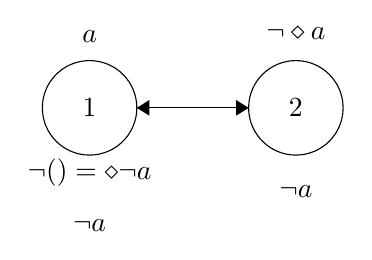
\begin{tikzpicture}[scale=0.2] \tikzstyle{every node}+=[inner sep=0pt] \draw [black] (26.7,-10.8) circle (3); \draw (26.7,-10.8) node {$1$};
\draw (26.7,-14.9) node {$\neg(\boxx{\dia})=\diamond\boxx{\neg a}$};
\draw (26.7,-18.3) node {$\neg a$}; \draw [black] (39.8,-10.8) circle (3); \draw (39.8,-10.8) node {$2$};
\draw (26.7,-6.3) node {$a$};
\draw (39.8,-6.1) node {$\neg\diamond a$};
\draw (39.8,-16.1) node {$\square\neg a$}; \draw [black] (29.7,-10.8) -- (36.8,-10.8); \fill [black] (36.8,-10.8) -- (36,-10.3) -- (36,-11.3); \draw [black] (36.8,-10.8) -- (29.7,-10.8); \fill [black] (29.7,-10.8) -- (30.5,-11.3) -- (30.5,-10.3); \end{tikzpicture} \end{center}

